\documentclass[12pt,a4paper,twoside]{book}
\usepackage[utf8]{inputenc}
\usepackage{graphicx}
\usepackage{xcolor}
\usepackage{amsmath}
\usepackage{tikz}
\usepackage[compat=1.1.0]{tikz-feynman}


\usepackage[left=2cm,right=2cm,top=2cm,bottom=2cm]{geometry}
\title{Appunti di interazioni fondamentali}
\author{Adriano Del Vincio}
\begin{document}
\maketitle

\section{Introduzione}
Questa è una raccolta di appunti tratta dalle lezioni del corso di interazioni fondamentali del professore Francesco Forti. 
L'intento è quello di seguire lo stile del corso in modo fedele. Tuttavia, di tanto in tanto, è presente qualche approfondimento. Tale caso sarà opportunamente segnalato con il simbolo \textcolor{blue}{*} ; il lettore potrà considerare tali argomenti facoltativi ad una prima lettura.
Nelle note sono presentati anche una serie di esercizi svolti, tratti dalle esercitazioni del professore Giovanni Signorelli. 
Gli argomenti sono divisi in moduli. I primi due riguardano esperimenti di fisica delle alte energie e cenni di rivelazione delle particelle. Nel modulo 2 si richiamano alcuni concetti di cinematica relativistica, si introduce lo spazio delle fasi e l'equazione di Dirac. \dots

\frontmatter
\tableofcontents 

\chapter{Modulo 2}\label{cap : Mod2}

\section{Richiami di cinematica relativistica}

Le leggi di trasformazione da un sistema di riferimento (s.r) che si muove con velocit\'a $\beta$ rispetto ad un altro sistema, lungo l'asse z, in relatività ristretta, sono le trasformazioni di Lorentz : 
\[
\begin{cases}
ct^{'}=\gamma (ct - \beta z) \\
x^{'}= x \\
y^{'}= y \\
z^{'}= \gamma z - \beta \gamma c t
\end{cases} 
\]

Per un generico \textit{boost} lungo una direzione qualunque specificata da $\beta = (\beta_{x}, \beta_{y}, \beta_{z})$ è più comodo utilizzare la seguente forma vettoriale :
\[
\begin{cases}
\frac{E^{'}}{c} = \gamma (\frac{E}{c} - \vec{\beta} \cdot \vec{p}) \\
\vec{p^{'}} =(\gamma - 1) \dfrac{( \vec{p} \cdot\vec{\beta}) \vec{\beta}}{\beta^{2}}  + \vec{p} - \beta \gamma \frac{E}{c}
\end{cases}
\]

Ricordiamo anche come cambia il concetto di simultaneità e contrazione delle lunghezze. Se abbiamo due eventi separati in un certo 
s.r con intervallo $\Delta t$, in un altro sistema di riferimento con velocità $\beta$ osserviamo $c \Delta t^{'} = \gamma c \Delta t - \beta \gamma \Delta z$. Quindi due eventi che avvengono simultaneamente in un sistema di riferimento, e sono separati spazialmente con distanza $\Delta z$, non sono simultanei in un altro sistema di riferimento che si muove con velocità $\beta$ rispetto al primo. 
Per la contrazione, dati due eventi nello spazio tempo con coordinate lungo l'asse z pari a $Z_a , Z_b$ in $O^{'}$, in un altro sistema $O$ che si muove rispetto al primo con velocità $\beta$ si ha $Z_{a}^{'} = \gamma Z_a$ e $Z_b^{'} = \gamma Z_b$. Perciò le distanza sono $\Delta Z^{'} = \gamma \Delta Z$ ovvero $\Delta Z = \frac{L}{\gamma}$. A questo punto è utile introdurre le formule di addizione delle velocità, ricavabili a partire dalle trasformazioni lungo z viste prima. Sapendo che in un sistema $S^{'}$ una particella si muove lungo z con velocità $u^{'}$, in un sistema $S$ un osservatore vedrà la particella muoversi con velocità:

\begin{equation}
u_z = \frac{\Delta Z}{\Delta t } = \dfrac{\gamma(\Delta Z^{'} + \beta c \Delta t ^{'})}{\gamma(c \Delta t^{'} + \beta \gamma \Delta z^{'})}  = \dfrac{\frac{u^{'}}{c} + \beta}{1 +  \frac{u^{'}}{c}\beta}
\end{equation}


Un altro risultato da tenere a mente: per una particella con vita media $\tau$ e con velocità $\beta$, si può ottenere il tempo di volo nel sistema di laboratorio semplicemente come $ t = \gamma \tau$, mentre l'ampiezza di volo sarà pari ad $\Delta l = \gamma \beta c  \tau$. 

\subsection{Quadrivettori}

E\' opportuno adesso richiamare la notazione di Einstein. In relatività ristretta il concetti di spazio e tempo sono profondamente connessi, per questo si introduce il concetto di vettore a 4 componenti $x^{\mu}$, o quadrivettore, in cui $x^{\mu = 0}$ è la componente temporale, mentre $x^{\mu = 1,2,3}$ sono le componenti spaziali. Un evento è rappresentato, in un certo sistema di riferimento, dal vettore $x^{\mu} = (ct, x , y, z)$ . Questa notazione permette di riscrive in modo estremamente compatto un boost nella direzione z 

\begin{equation}
x^{\mu'} = \sum _{\nu = 0}^{\nu = 3} \Lambda^\mu_\nu x^\nu 
\end{equation}
Dove con $\Lambda^\mu_\nu$:
\[
\begin{bmatrix}
\gamma & 0 & 0 & -\beta \gamma \\ 
0 & 1 & 0 & 0 \\ 
0 & 0 & 1 & 0 \\ 
- \beta \gamma & 0 & 0 & \gamma
\end{bmatrix} 
\]
In molti manuali, il simbolo di sommatoria è omesso, implicitamente si intende che si deve effettuare la somma sugli indici ripetuti (tranne nei casi in cui è specificato diversamente).
Una trasformazione di Lorentz può essere interpretata come una matrice di rotazione, che agisce in un spazio a 4-dimensioni. Si definisce adesso l'invariante di lorentz, ovvero:

\begin{equation*}
x^2 = (x^0)^2 - (x^1)^2 + (x^2)^2 + (x^3)^2 = (x^0)^2 - \vec{x} \cdot \vec{x}
\end{equation*}

Si può dimostrare che tale quantità è invariante rispetto alle trasformazioni di Lorentz, cioè assume lo stesso valore in tutti i sistemi di riferimento.
L'invariante di Lorentz si esprime in notazione di Einstein introducendo il tensore metrico $g_{\mu \nu}$ pari ad 
\begin{equation} \label{metric}
\begin{bmatrix}
1 & 0 & 0 & 0 \\ 
0 & -1 & 0 & 0 \\ 
0 & 0 & -1 & 0 \\ 
0 & 0 & 0 &-1
\end{bmatrix}
\end{equation} 
Con questo è possibile esprimere l'invariante di lorentz come $x^2 = x^\mu g_{\mu \nu} x^\nu $. In questa forma, è quasi immediato dimostrare che l'invariante di lorentz assume lo stesso valore in qualsiasi sistema di riferimento, è infatti sufficiente dimostrare, partendo da $x'^2 =  x'^\mu g_{\mu \nu} x'^\nu = x^\sigma \Lambda^\mu _\sigma g_{\mu \nu} \Lambda^\nu _\eta x^\eta $ che sia vera la relazione:  $ \Lambda^\mu _\sigma g_{\mu \nu} \Lambda^\nu _\eta = g_{\sigma \eta}$ 

\[
\begin{bmatrix}
\gamma & 0 & 0 & -\beta \gamma \\ 
0 & 1 & 0 & 0 \\ 
0 & 0 & 1 & 0 \\ 
- \beta \gamma & 0 & 0 & \gamma
\end{bmatrix} 
\cdot 
\begin{bmatrix}
1 & 0 & 0 & 0 \\ 
0 & -1 & 0 & 0 \\ 
0 & 0 & -1 & 0 \\ 
0 & 0 & 0 &-1
\end{bmatrix}
\cdot
\begin{bmatrix}
\gamma & 0 & 0 & -\beta \gamma \\ 
0 & 1 & 0 & 0 \\ 
0 & 0 & 1 & 0 \\ 
- \beta \gamma & 0 & 0 & \gamma
\end{bmatrix} 
=
\begin{bmatrix}
1 & 0 & 0 & 0 \\ 
0 & -1 & 0 & 0 \\ 
0 & 0 & -1 & 0 \\ 
0 & 0 & 0 &-1
\end{bmatrix}
\]

La scrittura $ x^\mu g_{\mu \nu} x^\nu$ può essere rielaborata introducendo il concetto di indice covariante e indice controvariante: $ x^\mu g_{\mu \nu} x^\nu = x^\mu x_\mu$ 
In questo caso abbiamo portato l'indice in alto $\nu$ in basso, dove $x_\nu = g_{\mu \nu} x^\nu$. Moltiplicando per  il tensore metrico è possibile alzare od abbassare gli indici, cioè trasformare un indice controvariante (come nel nostro caso) in un indice covariante e viceversa. In questi appunti la forma del tesore metrico è  quella scritta in equazione \ref{metric}, che è la metrica dello spazio-tempo di Minkowski. 

\subsection{Quadrimpulso, invarianti cinematici}

Oltre al quadrivettore $x^\mu$ che descrive la posizione nello spazio-tempo di una particella, si considera anche il quadrimpulso $P^\mu = (\frac{E}{c}, \vec{p})$. Le componenti del quadrimpulso sono legate dalla relazione:

\begin{equation*}
E = m \gamma c^2 \quad \vec{p} = m \gamma \beta c
\end{equation*}

Si ricava immediatamente che $ \frac{P^\mu}{m} = (\gamma c, \gamma \vec{v})$ che è la 4-velocità della particella. Alcune relazioni utili sono $\vec{\beta} = \frac{\vec{p} c}{E}$

\chapter{Modulo 3}
\chapter{modulo 4}
\chapter{Modulo 5}\label{cap : Mod5}

\section{DEEP INELASTIC SCATTERING \textcolor{blue}{*}}

In questo capitolo si analizzerà uno degli esperimenti che ha prodotto forti evidenze riguardo il modello a quark. Per \textit{deep inelastic scattering} si intende lo scattering tra elettrone e protone che avviene con un impulso trasferito elevato (sopra $1 Gev$). In tale regime si osserva un basso rate di collisioni elastiche, la maggior parte degli eventi produce un gran numero di adroni, si può quindi investigare la struttura interna del protone. Il deep inelastic scattering è analizzato considerando l'elettrone incidente interagisca con un quark libero del protone. Tale approssimazione può sembrare sorprendente, trascura infatti il legame forte tra i quark del protone. Giustificheremo tale fenomeno introducendo il concetto di \textbf{Asymptotic freedom} 

\subsection{SLAC-MIT experiment}

L'esperimento è stato condotto nel 1968 al Stanford Linear Accelerator (SLAC). Fasci di elettroni di energia $7-17 Gev$ venivano accelerati su bersagli di idrogeno (7 cm target). Il punto centrale dell'esperimento era la misura delle variabili cinematiche dell'elettrone uscente con precisione, determinando l'impulso trasferito al protone. L'impulso dell'elettrone veniva misurato tramite spettrometri magnetici, con la possibilità di ruotarli intorno al bersaglio per esplorare diversi angoli di scattering per gli elettroni uscenti. La configurazione dei detector permetteva la misura fino a $7.4 Gev$ di momento trasferito al protone.

\begin{figure}[hbtp]
\centering
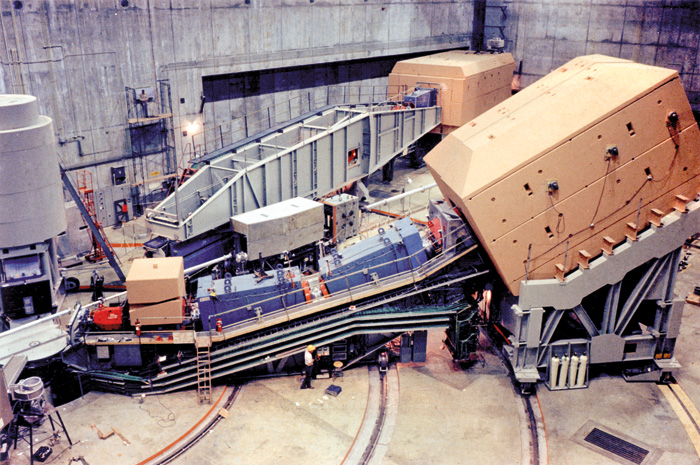
\includegraphics[scale=0.5]{CCsla3_09_12.jpg}
\caption{Struttura dell'esperimento, a destra si notato gli spettrometri con i calorimetri per discernere i pioni dagli elettroni. Il bersaglio di idrogeno è situato a sinistra, sotto il cilindro. Gli spettrometri potevano essere ruotati sui binari presenti in foto }
\end{figure}

Lo scopo dell'esperimento era quello di analizzare i costituenti interni del protone, ponendo attenzione alla misura dell'elettrone scatterato ed ignorando gli adroni nello stato finale. Il diagramma che descrive il processo 
\begin{center}

\feynmandiagram [horizontal=a to b] {
i1 [particle=\(e^{-}\)] -- [fermion] a -- [fermion] i2 [particle=\(e^{-}\)],
a -- [photon] b [blob],
f1 [particle=\(W\)]-- [anti fermion] b -- [anti fermion] f2 [particle=\(p\)] ,
};
\end{center}

Dove con $W$ indichiamo lo stato adronico finale. La corrente associata al vertice fotone-protone è un oggetto abbastanza complesso, bisogna fare alcune ipotesi, che portano sostanzialmente a formulare il modello a partoni, per poter scrivere l'ampiezza. Prima di procedere si fa un veloce richiamo al più semplice scattering elastico protone elettrone, studiato negli anni 50 da Robert Hofstadter a Stanford.

\paragraph{Sezione d'urto Rutherford}

Riportiamo velocemente una derivazione della sezione d'urto Rutherford utilizzando però gli opportuni limiti in teoria di campo. Nello scattering si ignora il rinculo del protone e si considera l'elettrone non relativistico. Gli spinori che descrivono il processo si scrivono :

\begin{equation}
\sqrt{E + m}\cdot
\left (\begin{array}{c}
• c \\ 
• s e^{i\phi} \\ 
• c K\\ 
• s K e^{i\phi}
\end{array} \right ) = 

\end{equation}
\chapter{modulo 6}
\end{document}